\documentclass[11pt,a4paper]{article}

% ---------------------------------------------------------------------------
%  AI Meets Control Theory -- living technical report
%  Rebuilt at every project milestone.  Owner: lava.
%  Build:  docs/report/build.sh   (or build.ps1 on Windows)
% ---------------------------------------------------------------------------

\usepackage[utf8]{inputenc}
\usepackage[T1]{fontenc}
\usepackage{lmodern}
\usepackage[margin=1in]{geometry}
\usepackage{amsmath,amssymb,amsfonts}
\usepackage{booktabs}
\usepackage{graphicx}
\usepackage{xcolor}
\usepackage{tikz}
\usetikzlibrary{arrows.meta,positioning,fit,backgrounds}
\usepackage{listings}
\usepackage{caption}
\usepackage{enumitem}
\usepackage[hidelinks]{hyperref}
\usepackage{fancyhdr}

\definecolor{aimctblue}{HTML}{0072B2}
\definecolor{aimctgreen}{HTML}{009E73}
\definecolor{aimctrust}{HTML}{D55E00}
\definecolor{codebg}{HTML}{F4F4F4}

\lstset{
  basicstyle=\ttfamily\small,
  backgroundcolor=\color{codebg},
  breaklines=true,
  frame=single,
  rulecolor=\color{lightgray},
  columns=fullflexible,
  keepspaces=true,
  language=Python,
  keywordstyle=\color{aimctblue}\bfseries,
  commentstyle=\color{aimctgreen},
  stringstyle=\color{aimctrust},
  showstringspaces=false,
}

\pagestyle{fancy}
\fancyhf{}
\rhead{\small AI Meets Control Theory}
\lhead{\small Living Technical Report}
\rfoot{\thepage}

\newcommand{\milestone}{M1 --- Phase~0 foundation}
\newcommand{\reportdate}{\today}

\title{\textbf{AI Meets Control Theory}\\[0.3em]
  \large From Classical Control to Intelligent Autonomous Systems\\[0.6em]
  \normalsize Living Technical Report --- \milestone}
\author{Generated by the project team (lead: puma; code: puma, toku; docs/research: lava, famo)}
\date{\reportdate}

\begin{document}
\maketitle
\thispagestyle{fancy}

\begin{abstract}
\noindent This report is regenerated at every project milestone. It documents
\emph{what the codebase can do}, \emph{the theory behind each component}, and
\emph{where the project currently stands}. The project is an open-source
laboratory for comparing classical control, optimal control, machine learning
and reinforcement learning on dynamical systems, under the principle:
\textit{build every method from scratch, simulate it, visualise it, and compare
it honestly}.
\end{abstract}

\tableofcontents
\bigskip

% ===========================================================================
\section{Introduction and Scope}
% ===========================================================================

The central question of the project is: \textbf{when should we use classical
control, when should we use AI, and when should we use both?} Rather than
assuming a neural network or an RL agent is the answer, every problem is first
attacked with PID, state feedback, LQR and MPC, and each method is measured
against the others on identical conditions.

Every topic follows the same cycle:
\begin{center}
Theory $\to$ Derivation $\to$ Implementation $\to$ Simulation\\
$\to$ Visualisation $\to$ Validation $\to$ Comparison $\to$ Experiment.
\end{center}

Fundamental algorithms are implemented from scratch in \texttt{numpy}; libraries
(\texttt{scipy}, \texttt{python-control}) are used only to cross-check.

% ===========================================================================
\section{Framework Architecture}
% ===========================================================================

The reusable library is the Python package \texttt{aimct} (\texttt{src/aimct/}).
Its design separates three concerns behind small interfaces so that any system,
any controller and the simulator compose freely.

\begin{figure}[h]
\centering
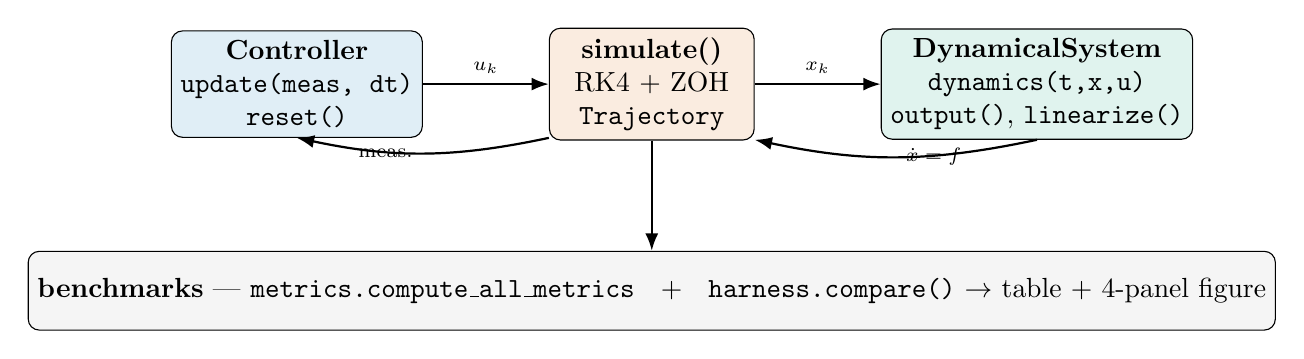
\begin{tikzpicture}[
  node distance=8mm and 16mm,
  box/.style={draw, rounded corners, align=center, minimum height=10mm,
              minimum width=26mm, fill=blue!5},
  sys/.style={box, fill=aimctgreen!12},
  ctl/.style={box, fill=aimctblue!12},
  sim/.style={box, fill=aimctrust!12},
  every edge/.style={draw, -{Latex[length=2.2mm]}, thick},
]
\node[ctl] (ctrl) {\textbf{Controller}\\ \texttt{update(meas, dt)}\\ \texttt{reset()}};
\node[sim, right=of ctrl] (sim) {\textbf{simulate()}\\ RK4 + ZOH\\ \texttt{Trajectory}};
\node[sys, right=of sim] (sysm) {\textbf{DynamicalSystem}\\ \texttt{dynamics(t,x,u)}\\ \texttt{output()}, \texttt{linearize()}};
\node[box, below=14mm of sim, fill=gray!8, minimum width=90mm] (bench)
     {\textbf{benchmarks} --- \texttt{metrics.compute\_all\_metrics} \; + \; \texttt{harness.compare()} $\rightarrow$ table + 4-panel figure};

\draw (ctrl) edge node[above,font=\scriptsize]{$u_k$} (sim);
\draw (sim) edge node[above,font=\scriptsize]{$x_{k}$} (sysm);
\draw (sysm.south) edge[bend left=12] node[right,font=\scriptsize]{$\dot x = f$} (sim.east|-sysm.south);
\draw (sim.west|-ctrl.south) edge[bend left=12] node[left,font=\scriptsize]{meas.} (ctrl.south);
\draw (sim) edge (bench);
\end{tikzpicture}
\caption{Core interfaces. The simulator drives a controller (\texttt{update(measurement, dt)})
and a system (\texttt{dynamics(t,x,u)}) through a fixed-step RK4 loop with
zero-order hold, returning aligned time/state/input/output arrays. Optional
hooks: \texttt{measurement\_fn} (what the controller sees) and
\texttt{input\_disturbance} (additive plant-input disturbance).}
\end{figure}

\subsection{Package layout}
\begin{lstlisting}[language=bash]
src/aimct/
  systems/      DynamicalSystem base + LinearSystem, MassSpringDamper,
                Pendulum, CartPole  (analytic Jacobians)
  simulate.py   rk4_step(), simulate() -> Trajectory(t, x, u, y)
  controllers/  Controller base + PID, StateFeedback, LQR
  benchmarks/   metrics.py (13 metrics), harness.py (compare())
  plot_style.py Okabe-Ito palette + canonical 4-panel comparison figure
  estimation/ ml/ rl/   (reserved for later phases)
\end{lstlisting}

% ===========================================================================
\section{Current Capabilities}
% ===========================================================================

\begin{table}[htbp]
\centering
\small
\begin{tabular}{@{}p{0.24\textwidth}p{0.40\textwidth}c@{}}
\toprule
\textbf{Component} & \textbf{What it provides} & \textbf{Tests} \\
\midrule
\texttt{systems} & Continuous-time models with a common
  \texttt{dynamics(t,x,u)} interface, full-state or custom output, and
  numerical \emph{and} analytic \texttt{linearize()}. Ships:
  linear SS, mass--spring--damper, pendulum, cart--pole. & \checkmark \\
\texttt{simulate} & Fixed-step RK4 with zero-order hold; \texttt{Trajectory}
  container; input saturation; measurement and disturbance hooks. & \checkmark \\
\texttt{PID} & From scratch: derivative-on-measurement with first-order
  filter, conditional-integration anti-windup, scalar or vector loops. & \checkmark \\
\texttt{StateFeedback} & Pole placement via Ackermann's formula (SISO). & \checkmark \\
\texttt{LQR} & Infinite-horizon regulator; CARE solved from scratch
  (Hamiltonian eigenvector method), cross-checked against
  \texttt{scipy.linalg.solve\_continuous\_are}. & \checkmark \\
\texttt{benchmarks.metrics} & 13 step-response / effort metrics: rise \&
  settling time, overshoot, $e_{ss}$, RMSE, IAE, ITAE, ISE, control energy,
  peak, slew, saturation duty. & \checkmark \\
\texttt{benchmarks.harness} & \texttt{compare()} runs $N$ controllers on one
  system under identical conditions, emits the standard Markdown/CSV table and
  the 4-panel figure. & \checkmark \\
\bottomrule
\end{tabular}
\caption{Implemented as of \milestone. See \texttt{docs/roadmap.md} for what is next.}
\end{table}

% ===========================================================================
\section{Theory: Modelling and Simulation}
% ===========================================================================

A system is a first-order ODE $\dot x = f(t,x,u)$ with output $y = g(t,x,u)$.
Second-order mechanics are written in state form, e.g. the mass--spring--damper
$m\ddot q + c\dot q + k q = u$ becomes
\[
\frac{d}{dt}\begin{bmatrix} q \\ \dot q \end{bmatrix}
= \begin{bmatrix} 0 & 1 \\ -k/m & -c/m \end{bmatrix}
  \begin{bmatrix} q \\ \dot q \end{bmatrix}
+ \begin{bmatrix} 0 \\ 1/m \end{bmatrix} u .
\]

\paragraph{Linearisation.} About an equilibrium $(x_e,u_e)$,
$A = \left.\partial f/\partial x\right|_{e}$, $B = \left.\partial f/\partial u\right|_{e}$.
The base class provides a central-difference Jacobian; each concrete system also
supplies the closed-form $A,B$ (the test suite asserts the two agree).

\paragraph{Integration.} The simulator advances the state with classical
fourth-order Runge--Kutta,
\[
x_{k+1} = x_k + \tfrac{h}{6}\left(k_1 + 2k_2 + 2k_3 + k_4\right),
\]
holding $u$ constant across each step (zero-order hold), which matches how a
discrete-time controller actually drives a plant.

% ===========================================================================
\section{Theory: Classical Control --- PID}
% ===========================================================================

The control law
$u(t) = K_p e(t) + K_i \!\int_0^t\! e\,d\tau + K_d \dot d(t)$, with
$e = r - y$, and the derivative acting on a filtered measurement to avoid
derivative kick. Discrete form with step $h$:
\[
I_k = I_{k-1} + e_k h, \quad
D_k = D_{k-1} + \frac{h}{\tau_d + h}\big(D^{\text{raw}}_k - D_{k-1}\big), \quad
u_k = K_p e_k + K_i I_k + K_d D_k .
\]
Under saturation, \emph{conditional integration} freezes $I_k$ whenever the
unsaturated command is outside the limits and the error would push it further
out --- preventing windup.

\subsection{Worked example: stabilising an unstable plant (Experiment 03)}

Plant with a right-half-plane pole, $\ddot y - \omega_0^2 y = u + d$,
$\omega_0 = 2$, unit step reference, step input disturbance $d=0.5$ at $t=5$\,s,
actuator limit $|u|\le 10$.

\begin{itemize}[nosep]
  \item \textbf{P-only} cannot stabilise it: the closed loop is
        $s^2 + (K_p-\omega_0^2)$ --- poles on the imaginary axis, and once the
        actuator saturates on this unstable plant the response diverges.
  \item \textbf{PD} places both poles in the left half-plane, but the
        closed-loop DC gain from $r$ is $K_p/(K_p-\omega_0^2) = 20/16 = 1.25$,
        so PD tracks the step with a permanent \textbf{25\% offset}.
  \item \textbf{PID} removes the steady-state error for both the step and the
        disturbance.
  \item \textbf{Anti-windup} on the same gains cuts overshoot from
        $53\% \to 39\%$ and IAE from $0.93 \to 0.80$.
\end{itemize}

\begin{figure}[h]
\centering
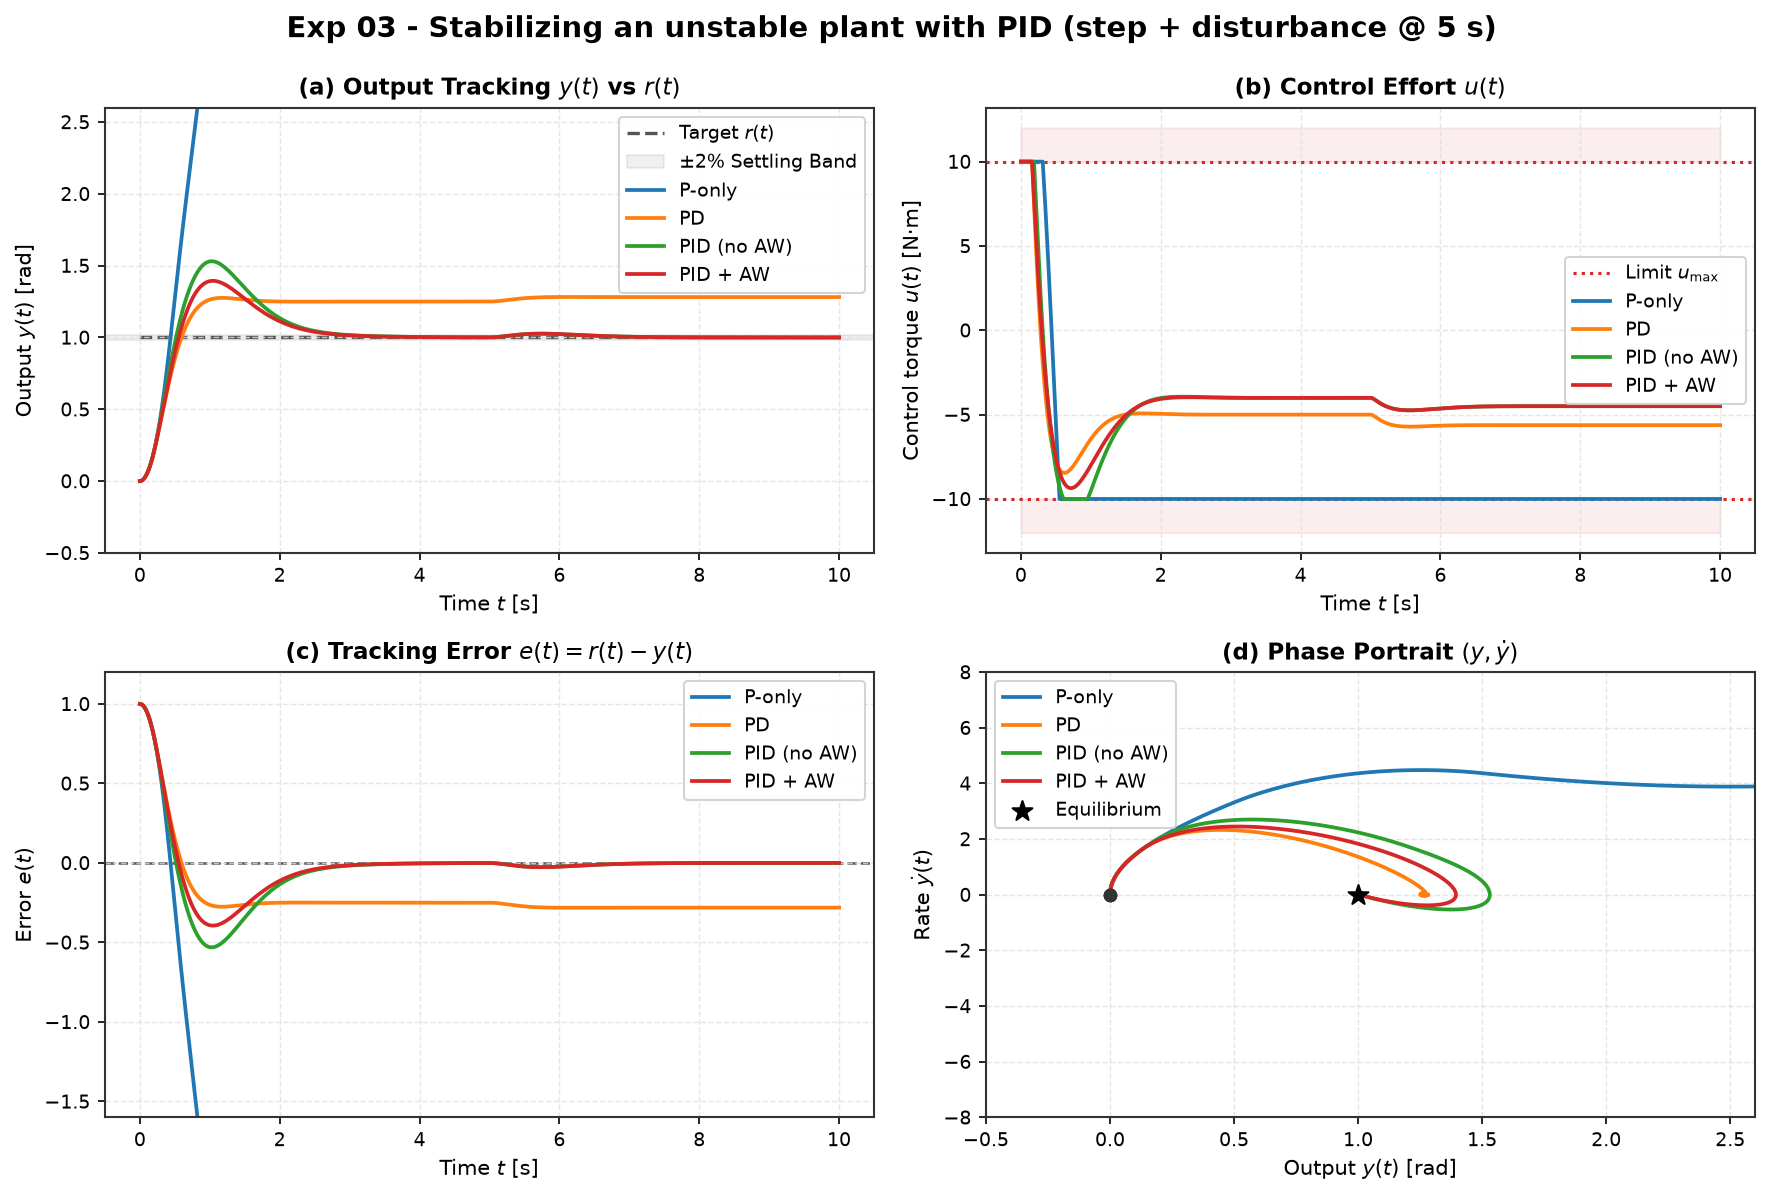
\includegraphics[width=\textwidth]{figures/exp03_pid_unstable.png}
\caption{Experiment 03 --- P / PD / PID / PID+anti-windup on the unstable
second-order plant. Panels: (a) output tracking, (b) control effort with the
actuator limit, (c) tracking error, (d) phase portrait. Regenerated from
\texttt{experiments/03\_pid\_stabilizes\_unstable/run.py}.}
\end{figure}

% ===========================================================================
\section{Theory: Modern Control --- Pole Placement and LQR}
% ===========================================================================

For $\dot x = Ax + Bu$ with $(A,B)$ controllable, state feedback $u = -Kx$ can
place the closed-loop eigenvalues of $A - BK$ anywhere. \texttt{StateFeedback}
uses Ackermann's formula. \texttt{LQR} instead \emph{chooses} the poles
implicitly by minimising
\[
J = \int_0^\infty \big(x^\top Q x + u^\top R u\big)\,dt ,
\qquad u = -R^{-1}B^\top P\, x ,
\]
where $P$ solves the continuous-time algebraic Riccati equation
$A^\top P + P A - P B R^{-1} B^\top P + Q = 0$. We solve it from scratch via the
stable invariant subspace of the Hamiltonian
$\left[\begin{smallmatrix} A & -BR^{-1}B^\top \\ -Q & -A^\top \end{smallmatrix}\right]$,
and verify the residual and the \texttt{scipy} solution agree.

% ===========================================================================
\section{Project Status and Roadmap}
% ===========================================================================

\paragraph{Milestone \milestone{} --- done.} Library skeleton, four reference
systems, RK4 simulator, PID / StateFeedback / LQR, metrics, comparison harness,
Experiment 03, CI on Python 3.10--3.12, module 01--05 theory notes.

\paragraph{Next.}
\begin{itemize}[nosep]
  \item Experiment 04: LQR vs pole placement vs PID on the cart--pole.
  \item Module 04--05 notes paired with the new controllers.
  \item Observers + Kalman filter (\texttt{estimation/}).
  \item From-scratch linear MPC with constraints (Phase~2).
\end{itemize}

\paragraph{Reproduce.}
\begin{lstlisting}[language=bash]
pip install -e ".[dev,xcheck]"
pytest -q
python experiments/03_pid_stabilizes_unstable/run.py
\end{lstlisting}

\end{document}
